\documentclass[a4paper,12pt]{article}
\usepackage{graphicx}
\usepackage{float}
\usepackage{listings}
\usepackage{color}
\usepackage{courier}
\usepackage{geometry}
\geometry{margin=1in}
\usepackage{enumitem}
\usepackage{titlesec}

% Define Java syntax highlighting
\definecolor{javared}{rgb}{0.6,0,0}
\definecolor{javagreen}{rgb}{0.25,0.5,0.35}
\definecolor{javapurple}{rgb}{0.5,0,0.35}
\definecolor{javadocblue}{rgb}{0.25,0.35,0.75}
\lstset{
    language=Java,
    basicstyle=\ttfamily\small,
    keywordstyle=\color{javared}\bfseries,
    stringstyle=\color{javagreen},
    commentstyle=\color{javagreen}\itshape,
    morecomment=[s][\color{javadocblue}]{/**}{*/},
    numbers=left,
    numberstyle=\tiny\color{black},
    stepnumber=1,
    numbersep=10pt,
    tabsize=4,
    showspaces=false,
    showstringspaces=false
}

% Custom command for practical title
\newcounter{practicalno} % Create a new counter for practical numbers
\setcounter{practicalno}{-1} % Initialize the counter to 0
\newcommand{\practicaltitle}[1]{
    \stepcounter{practicalno} % Increment the practical number counter
    \newpage
    \begin{center}
        \vspace{1cm}
        \Large\textbf{Practical \thepracticalno} \\
        \vspace{0.5cm}
        \Large\textbf{#1} % Display the title on the next line
        \normalsize\vspace{1cm}
    \end{center}
}

%Redefine \subsection command to use hashtags instead of numbers
\titleformat{\subsection}[block]{\bfseries\large}{\texttt{\#}}{1em}{}
% Redefine \subsubsection command to use arrow instead of numbers
\titleformat{\subsubsection}[block]{\bfseries\normalsize}{\texttt{>}}{1em}{}

\title{\textbf{Java Practical}}
\author{Mayank}
\date{}

% Redefine \subsection command to use hashtags instead of numbers
\titleformat{\subsection}[block]{\bfseries\large}{\texttt{\#}}{1em}{}

\begin{document}

\maketitle

\practicaltitle{Introduction to Java}

\section{Introduction to Java}
JAVA was developed by James Gosling at Sun Microsystems Inc in May 1995 and later acquired by Oracle Corporation. It is a simple programming language. Java makes writing, compiling, and debugging programming easy. It helps to create reusable code and modular programs. Java is a class-based, object-oriented programming language and is designed to have as few implementation dependencies as possible. A general-purpose programming language made for developers to write once run anywhere that is compiled Java code can run on all platforms that support Java. Java applications are compiled to byte code that can run on any Java Virtual Machine. The syntax of Java is similar to C/C++.

Java is widely used for developing applications for desktop, web, and mobile devices. Java is known for its simplicity, robustness, and security features, making it a popular choice for enterprise-level applications.

\section{Java Syntax}
Java syntax is the set of rules defining how a Java program is written and interpreted.
\subsubsection{Code: }
\begin{lstlisting}
public class Syntax {
    public static void main(String[] args) {
        System.out.println("Hello, World!");
    }
}
\end{lstlisting}

% \subsection{Output: }
% \begin{}
%     \fbox{
%         \parbox{0.9\linewidth}{
%             \centering
%             \texttt{Hello, World!}
%         }
%     }
% \end{}

\subsection*{public class Main}
\begin{itemize}[leftmargin=2cm]
    \item \textbf{public}: An access modifier indicating that the class is accessible from other classes.
    \item \textbf{class}: A keyword used to define a class in Java.
    \item \textbf{Main}: The name of the class. By convention, class names in Java start with an uppercase letter.
\end{itemize}

\subsection*{public static void main(String[] args)}
\begin{itemize}[leftmargin=2cm]
    \item \textbf{static}: A keyword indicating that the method belongs to the class, not to instances of the class. It can be called without creating an object of the class.
    \item \textbf{void}:  The return type of the method, indicating that it does not return any value.
    \item \textbf{main}: The name of the method. This is the entry point of any Java application.
    \item \textbf{String[] args}: An array of String arguments passed to the method. These are command-line arguments.
\end{itemize}

\subsection*{System.out.println("Hello, World!")}
\begin{itemize}[leftmargin=2cm]
    \item \textbf{System}: A built-in class in the \texttt{java.lang} package.
    \item \textbf{out}: A static field in the \textbf{System} class, which is an instance of \textbf{PrintStream}.
    \item \textbf{println}: A method of \textbf{PrintStream} that prints a message to the standard output (usually the console) followed by a newline.
    \item \textbf{"Hello, World!"}: A string literal that is the message to be printed.
\end{itemize}


\section{Variables in Java}
Variables are containers for storing data values. In Java, every variable must be declared before it is used. A variable declaration includes the data type followed by the variable name. Java supports different types of variables, including:
\begin{itemize}[leftmargin=2cm]
    \item \textbf{Local Variables}: Declared inside a method and accessible only within that method.
    \item \textbf{Instance Variables}: Declared inside a class but outside any method. They are accessible from any method in the class.
    \item \textbf{Static Variables}: Declared with the \texttt{static} keyword. These are shared among all instances of the class.
\end{itemize}


\setcounter{section}{0}
\practicaltitle{Handling Various Data Types}

\section{Data Types in Java}
Java has two categories of data types: \textbf{Primitive Data Types} and \textbf{Reference/Object Data Types}.

\subsection{Primitive Data Types}
Primitive data types are the most basic data types available in Java.
\subsubsection{Code: }
\begin{lstlisting}
public class Data {
    public static void main(String[] args) {
        int myNum = 5;               
        float myFloatNum = 5.99f;
        double myDoubNum = 5.9999d;  
        char myLetter = 'D';        
        boolean myBool = true;       
        String myText = "Hello";     

        System.out.println(myNum);
        System.out.println(myFloatNum);
        System.out.println(myDoubNum);
        System.out.println(myLetter);
        System.out.println(myBool);
        System.out.println(myText);
    }
}
\end{lstlisting}

\begin{figure}[H]
    \centering
    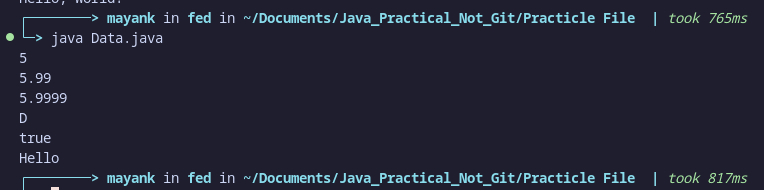
\includegraphics[width=0.9\linewidth]{images/DataOutput.png}
    \caption{Primitve Data Types}
    \label{fig:sample_image}
\end{figure}

\begin{itemize}[leftmargin=2cm]
    \item \textbf{byte}: 8-bit signed integer. Range: -128 to 127.
    \item \textbf{short}: 16-bit signed integer. Range: -32,768 to 32,767.
    \item \textbf{int}: 32-bit signed integer. Range: -2\textsuperscript{31} to 2\textsuperscript{31}-1.
    \item \textbf{long}: 64-bit signed integer. Range: -2\textsuperscript{63} to 2\textsuperscript{63}-1.
    \item \textbf{float}: 32-bit floating-point number.
    \item \textbf{double}: 64-bit floating-point number.
    \item \textbf{char}: 16-bit Unicode character.
    \item \textbf{boolean}: Represents two values: true and false.
\end{itemize}

\subsection{Non Primitive Data Types}
Reference types in Java are Strings and arrays:
\subsubsection{Code: }
\begin{lstlisting}
public class NonPrimitive {
    public static void main(String[] args) {
        // String Data Type
        String stringVar = "Hello, Java!";
        System.out.println("\nString Data Type:");
        System.out.println("String: " + stringVar);

        // Array Data Type
        int[] intArray = {1, 2, 3, 4, 5};
        System.out.println("\nArray Data Type:");
        System.out.print("intArray: ");
        for (int num : intArray) {
            System.out.print(num + " ");
        }
        System.out.println();
    }
}  
\end{lstlisting}

\begin{figure}[H]
    \centering
    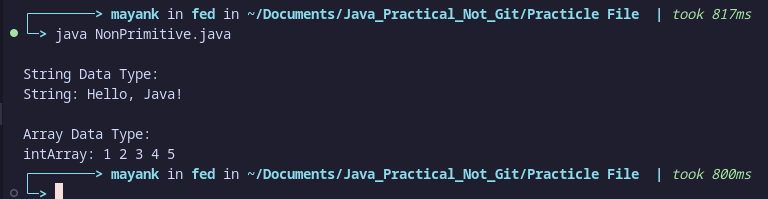
\includegraphics[width=0.9\linewidth]{images/NonPrimData.png}
    \caption{Non-Primitve Data Types}
    \label{fig:sample_image}
\end{figure}

\begin{itemize}[leftmargin=2cm]
    \item \textbf{Strings}: Sequences of characters.
    \item \textbf{Arrays}: Containers that hold multiple values of the same type.
\end{itemize}

\setcounter{section}{0}

% \practicaltitle{Practical 2: Type casting}
\practicaltitle{Type casting}
Type casting is when you assign a value of one primitive data type to another type. There are two types of type casting, implicit typecasting and explicit typecasting which are explained below:

\section{Implicit Type Casting}
Implicit type casting is done automatically when passing a smaller size type to a larger size type.
\begin{center}
    \fbox{
        \parbox{0.9\linewidth}{
            \centering
            \texttt{byte $\rightarrow$ short $\rightarrow$ char $\rightarrow$ int $\rightarrow$ long $\rightarrow$ float $\rightarrow$ double}
        }
    }
\end{center}
\subsubsection{Code: }
\begin{lstlisting}
public class Implicit {
    public static void main(String[] args) {
        int myInt = 9;
        double myDouble = myInt; // Automatic casting: int to double
        System.out.println(myInt); // Outputs 9
        System.out.println(myDouble); // Outputs 9.0
    }
}    
\end{lstlisting}
\subsubsection{Output: }
\begin{figure}[H]
    \centering
    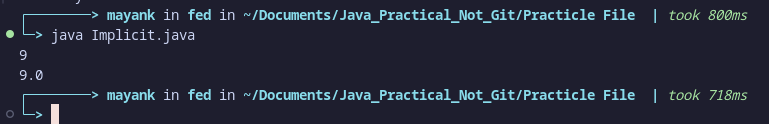
\includegraphics[width=0.9\linewidth]{images/ImplicitOut.png}
    \caption{Implicit Type Conversion}
    \label{fig:sample_image}
\end{figure}

\section{Explicit Type Casting}
Explicit type casting must be done manually by placing the type in parentheses () in front of the value.
\begin{center}
    \fbox{
        \parbox{0.9\linewidth}{
            \centering
            \texttt{double $\rightarrow$ float $\rightarrow$ long $\rightarrow$ int $\rightarrow$ char $\rightarrow$ short $\rightarrow$ byte}
        }
    }
\end{center}
\begin{lstlisting}
public class Explicit {
    public static void main(String[] args) {
        double myDouble = 9.78d;
        int myInt = (int) myDouble; // Manual casting: double to int
    
        System.out.println(myDouble);   // Outputs 9.78
        System.out.println(myInt);      // Outputs 9
    }
}
\end{lstlisting}
\subsubsection{Output: }
\begin{figure}[H]
    \centering
    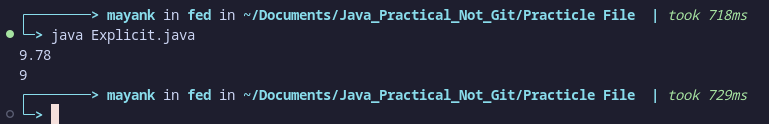
\includegraphics[width=0.9\linewidth]{images/ExplicitOut.png}
    \caption{Explicit Type Conversion}
    \label{fig:sample_image}
\end{figure}

\setcounter{section}{0}

\practicaltitle{Array 1D and 2D}

\section{1-Dimensional Array}
Arrays are used to store multiple values in a single variable, instead of declaring separate variables for each value.
\subsubsection{Code: }
\begin{lstlisting}
public class Array {
    public static void main(String[] args) {
        String[] cars = {"Volvo", "BMW", "Ford", "Mazda"};
        System.out.println(cars[0]); 
        System.out.println(cars[1]); 
        System.out.println(cars[2]); 
        System.out.println(cars[3]); 
        // Changing an element of an array
        cars[0] = "audi";
        System.out.println(cars[0]); 
        // Length of an array
        System.out.println(cars.length);
        // Loop through an array
        for (String arr  : cars) {
            System.out.println(arr);
        }
    }
}  
\end{lstlisting}
\subsubsection{Output: }
\begin{figure}[H]
    \centering
    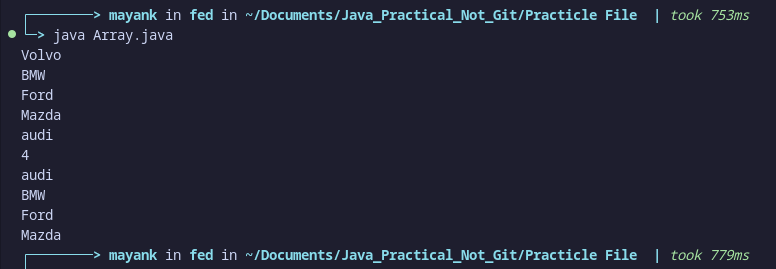
\includegraphics[width=0.9\linewidth]{images/output2.png}
    \caption{output of 1-D array}
    \label{fig:sample_image}
\end{figure}

\section{Multi Dimensional Array}
A multidimensional array is an array of arrays. Multidimensional arrays are useful when you want to store data as a tabular form, like a table with rows and columns.
\subsubsection{Code: }
\begin{lstlisting}
    // Program for Multi-Dimensional Array

public class Array2D {
    public static void main(String[] args) {
        int[][] my2DArr = {{10, 20, 30, 40}, {50, 60, 70}};
        // Accessing Elemensts of array
        System.out.println(my2DArr[0][0]); // 10
        System.out.println(my2DArr[1][2]); // 70
        // change element of array
        my2DArr[0][0] = 100;
        System.out.println(my2DArr[0][0]); //100

        // Loop through a multi dimensional array
        System.out.println("Looping through an array");
        for (int[] row : my2DArr) {
            for(int i : row) {
                System.out.println(i);
            }
        }
    }
}
  
\end{lstlisting}
\subsubsection{Output: }
\begin{figure}[H]
    \centering
    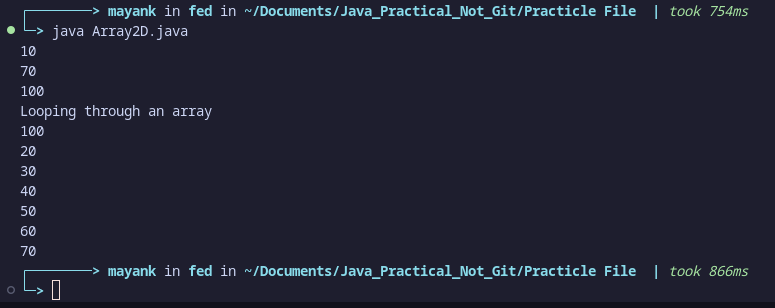
\includegraphics[width=0.9\linewidth]{images/output3.png}
    \caption{output of Multi-D array}
    \label{fig:sample_image}
\end{figure}

\setcounter{section}{0}

\practicaltitle{Various Control Strucutures}

\section{For loop}
For loop provides a concise way of writing the loop structure. Unlike a while loop, a
for statement consumes the initialization, condition and increment/decrement in one line
thereby providing a shorter, easy to debug structure of looping.
\subsubsection{Code: }
\begin{lstlisting}
import java.util.Scanner;

public class ForLoop {

    public static void main(String[] args) {
        Scanner sc = new Scanner(System.in);
        System.out.print("Enter a number: ");
        int n = sc.nextInt();
        for (int i = 0; i < n; i++) {
            System.out.print(i + " ");
        }
        System.out.println();
    }
}
\end{lstlisting}
\subsubsection{Output: }
\begin{figure}[H]
    \centering
    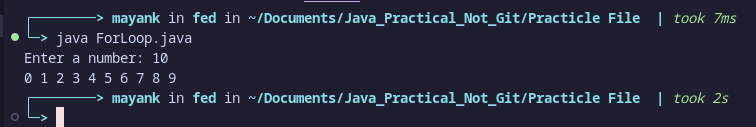
\includegraphics[width=0.9\linewidth]{images/ForOut.png}
    \caption{output of for loop}
    \label{fig:sample_image}
\end{figure}

\section{While loop}
A while loop is a control flow statement that allows code to be executed repeatedly
based on a given Boolean condition. The while loop can be thought of as a repeating if
statement.
\subsubsection{Code: }
\begin{lstlisting}
import java.util.Scanner;

public class WhileLoop {

    public static void main(String[] args) {
// Sum of first n numbers
        Scanner sc = new Scanner(System.in);
        System.out.print("Enter a number: ");
        int n = sc.nextInt();
        int sum = 0;
        while (n > 0) {
            sum += n--;
        }
        System.out.println(sum);
    }
}
\end{lstlisting}
\subsubsection{Output: }
\begin{figure}[H]
    \centering
    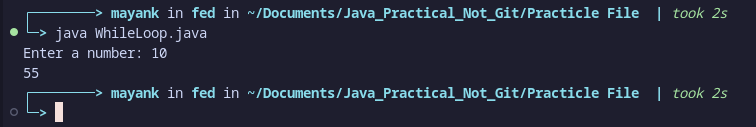
\includegraphics[width=0.9\linewidth]{images/WhileOut.png}
    \caption{output of while loop}
    \label{fig:sample_image}
\end{figure}

\section{Do-While loop}
Do-While loop is similar to while loop with only difference that it checks for condition
after executing the statements, and therefore is an example of Exit Control Loop.
\subsubsection{Code: }
\begin{lstlisting}
import java.util.Scanner;

public class DoWhile {

    public static void main(String[] args) {
// Sum of first n numbers
        Scanner sc = new Scanner(System.in);
        System.out.print("Enter a number: ");
        int n = sc.nextInt();
        int sum = 0;
        do {
            sum += n--;
        } while (n > 0);
        System.out.println(sum);
    }
}
\end{lstlisting}
\subsubsection{Output: }
\begin{figure}[H]
    \centering
    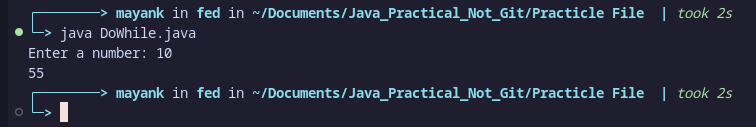
\includegraphics[width=0.9\linewidth]{images/image.png}
    \caption{output of do-while loop}
    \label{fig:sample_image}
\end{figure}

\setcounter{section}{0}

\practicaltitle{Various Decision Strucutures}

\section{The IF statement}
Use the if statement to specify a block of Java code to be executed if a condition is true.
\subsubsection{Code: }
\begin{lstlisting}
public class If {
    public static void main(String[] args) {
        if (20 > 18) {
            System.out.println("20 is greater than 18");
        }
    }
}    
\end{lstlisting}
\subsubsection{Output: }
\begin{figure}[H]
    \centering
    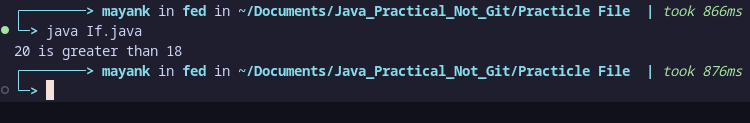
\includegraphics[width=0.9\linewidth]{images/output4.png}
    \caption{output of if statement}
    \label{fig:sample_image}
\end{figure}

\section{The IF-Else statement}
Executes one block of code if its condition evaluates to true, and another block of code if it evaluates to false.
\subsubsection{Code: }
\begin{lstlisting}
public class IfElse {
    public static void main(String[] args) {
        int time = 20;
        if (time < 18) {
            System.out.println("Good day.");
        } else {
            System.out.println("Good evening.");
        }
    }
}    
\end{lstlisting}
\subsubsection{Output: }
\begin{figure}[H]
    \centering
    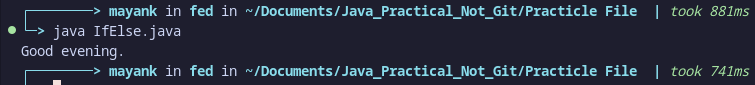
\includegraphics[width=0.9\linewidth]{images/output5.png}
    \caption{output of if-else statement}
    \label{fig:sample_image}
\end{figure}

\section{The IF-Else ladder}
Executes one block of code if its condition evaluates to true, and then checks other
coditions given in else if statements if it is false, or executes the last else block if nothing
is true
\subsubsection{Code: }
\begin{lstlisting}
import java.util.Scanner;

public class IfElseLad {

    public static void main(String[] args) {
        Scanner sc = new Scanner(System.in);
        System.out.print("Enter age -> ");
        int age = sc.nextInt();
        if (age < 12) {
            System.out.println("Child"); 
        }else if (age < 18) {
            System.out.println("Teenager"); 
        }else {
            System.out.println("Adult");
        }
    }
}

    \end{lstlisting}
\subsubsection{Output: }
\begin{figure}[H]
    \centering
    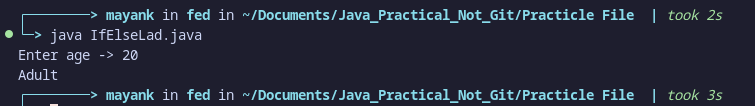
\includegraphics[width=0.9\linewidth]{images/IfElseLad.png}
    \caption{output of if-else-ladder statement}
    \label{fig:sample_image}
\end{figure}

\section{Nested If-Else}
We can put If-Else statements inside otehr If-Else statemetns in order to build more
complex logic
\subsubsection{Code: }
\begin{lstlisting}
import java.util.Scanner;

public class NestedIf {

    public static void main(String[] args) {
        Scanner sc = new Scanner(System.in);
        System.out.print("Enter a -> ");
        int a = sc.nextInt();
        System.out.print("Enter b -> ");
        int b = sc.nextInt();
        System.out.print("Enter c -> ");
        int c = sc.nextInt();
        if (a > b) {
            if (a > c) {
                System.out.println("A is greatest"); 
            }else {
                System.out.println("C is greatest");
            }
        } else {
            if (b > c) {
                System.out.println("B is greatest"); 
            }else {
                System.out.println("C is greatest");
            }
        }
    }
}    
\end{lstlisting}
\subsubsection{Output: }
\begin{figure}[H]
    \centering
    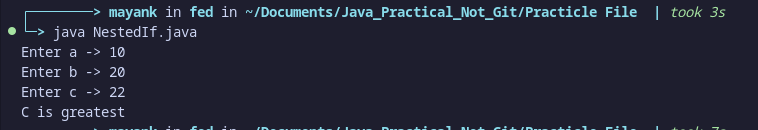
\includegraphics[width=0.9\linewidth]{images/NestOut.png}
    \caption{output of nested-if statement}
    \label{fig:sample_image}
\end{figure}

\section{Switch statement}
The switch statement in Java is a multi-way branch statement. In simple words, the Java
switch statement executes one statement from multiple conditions.
\subsubsection{Code: }
\begin{lstlisting}
import java.util.Scanner;

public class Switch {

    public static void main(String[] args) {
        Scanner sc = new Scanner(System.in);
        System.out.print("Enter a number: ");
        int day = sc.nextInt();
        switch (day) {
            case 1:
                System.out.println("Sunday");
                break;
            case 2:
                System.out.println("Monday");
                break;
            case 3:
                System.out.println("Tuesday");
                break;
            case 4:
                System.out.println("Wednesday");
                break;
            case 5:
                System.out.println("Thursday");
                break;
            case 6:
                System.out.println("Friday");
                break;
            case 7:
                System.out.println("Saturday");
                break;
            default:
                System.out.println("Invalid day");
        }
    }
}
    
\end{lstlisting}
\subsubsection{Output: }
\begin{figure}[H]
    \centering
    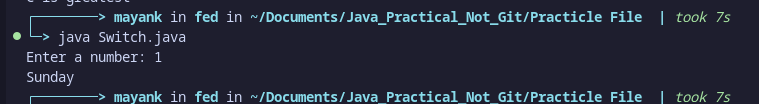
\includegraphics[width=0.9\linewidth]{images/SwitchOut.png}
    \caption{output of switch statement}
    \label{fig:sample_image}
\end{figure}

\setcounter{section}{0}

% \practicaltitle{Practical 2: Type casting}
\practicaltitle{Recursion}
Recursion is the technique of making a function call itself. This technique provides a way to break complicated problems down into simple problems which are easier to solve.

\section{Example of Recursion}
\subsection{Code: }
\begin{lstlisting}
public class Recursion {
    public static void main(String[] args) {
        int result = sum(10);
        System.out.println(result);
    }
    public static int sum(int k) {
        if (k > 0) {
        return k + sum(k - 1);
        } else {
        return 0;
        }
    }
}
\end{lstlisting}
\subsubsection{Output: }
\begin{figure}[H]
    \centering
    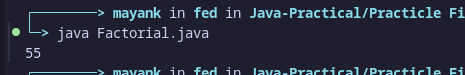
\includegraphics[width=0.9\linewidth]{images/RecExp.png}
    \caption{Recursion Example}
    \label{fig:sample_image}
\end{figure}

\section{Factorial of a number using Recursion}
\subsection{Code: }
\begin{lstlisting}
public class Factorial {
    static int factorial(int n)
    {
        if (n == 0 || n == 1)
            return 1;
        return n * factorial(n - 1);
    }
    public static void main(String[] args)
    {
        int ans = factorial(5);
        System.out.println("Factorial of 5 is :" + ans);
    }
}   
\end{lstlisting}
\subsubsection{Output: }
\begin{figure}[H]
    \centering
    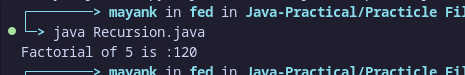
\includegraphics[width=0.9\linewidth]{images/RecursionOut.png}
    \caption{Factorial using example}
    \label{fig:sample_image}
\end{figure}

\setcounter{section}{0}

% \practicaltitle{Practical 2: Type casting}
\practicaltitle{Method Overloading by passing objects as arguments}
In object-oriented programming, method overloading is a feature that allows you to define multiple methods with the same name but different parameters. In the context of passing objects as arguments, method overloading can be used to handle different types or classes of objects.

\section{Example of Method Overloading by passing objects as arguments}
\subsection{Code: }
\begin{lstlisting}
class Circle {
    double radius;
    Circle(double radius) {
        this.radius = radius;
    }
}

class Rectangle {
    double length, width;
    Rectangle(double length, double width) {
        this.length = length;
        this.width = width;
    }
}

class AreaCalculator {
    double calculateArea(Circle circle) {
        return Math.PI * circle.radius * circle.radius;
    }
    double calculateArea(Rectangle rectangle) {
        return rectangle.length * rectangle.width;
    }
}
public class MOPOAA {
    public static void main(String[] args) {
        Circle circle = new Circle(5);
        Rectangle rectangle = new Rectangle(4, 6);
        AreaCalculator calculator = new AreaCalculator();
        System.out.println
        ("Area of Circle: "+calculator.calculateArea(circle));
        System.out.println
        ("Area of Rectangle:"+calculator.calculateArea(rectangle));
    }
}    
\end{lstlisting}
\subsubsection{Output: }
\begin{figure}[H]
    \centering
    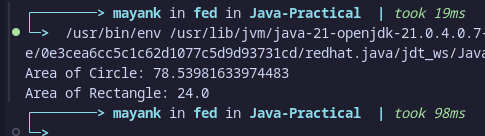
\includegraphics[width=0.9\linewidth]{images/MOPOAA.png}
    \caption{Method Overloading by passing objects as arguments}
    \label{fig:sample_image}
\end{figure}

\setcounter{section}{0}

% \practicaltitle{Practical 2: Type casting}
\practicaltitle{Constructor Overloading by passing objects as arguments}
Constructor overloading in object-oriented programming allows a class to have multiple constructors with different parameter lists. This enables the creation of objects in different ways. When you overload constructors by passing objects as arguments, you can create new objects based on existing objects.

\section{Example of Constructor Overloading by passing objects as arguments}
\subsection{Code: }
\begin{lstlisting}
class Book {
    String title;
    String author;
    int pages;
    // Constructor 1: No arguments
    Book() {
        this.title = "Unknown";
        this.author = "Unknown";
        this.pages = 0;
    }
    // Constructor 2: Passing title, author, and pages
    Book(String title, String author, int pages) {
        this.title = title;
        this.author = author;
        this.pages = pages;
    }
    /*
    Constructor 3: Passing an existing Book object
    (copy constructor)
    */
    Book(Book existingBook) {
        this.title = existingBook.title;
        this.author = existingBook.author;
        this.pages = existingBook.pages;
    }
    void displayDetails() {
        System.out.println("Title: " + title);
        System.out.println("Author: " + author);
        System.out.println("Pages: " + pages);
    }
}
public class COBPOAA {
    public static void main(String[] args) {
        // Using Constructor 1
        Book book1 = new Book();
        System.out.println("Book 1 details:");
        book1.displayDetails();

        // Using Constructor 2
        Book book2 = new Book("1984", "George Orwell", 328);
        System.out.println("\nBook 2 details:");
        book2.displayDetails();

        // Using Constructor 3 (Copy Constructor)
        Book book3 = new Book(book2);
        System.out.println
        ("\nBook 3 details (copied from Book 2):");
        book3.displayDetails();
    }
}    
\end{lstlisting}
\subsubsection{Output: }
\begin{figure}[H]
    \centering
    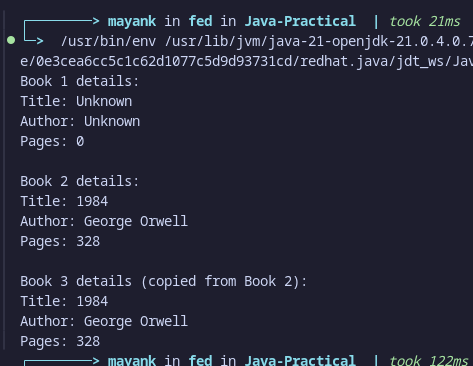
\includegraphics[width=0.9\linewidth]{images/COBPAA.png}
    \caption{Constructor Overloading by passing objects as arguments}
    \label{fig:sample_image}
\end{figure}

\setcounter{section}{0}

% \practicaltitle{Practical 2: Type casting}
\practicaltitle{Command Line Arguments}
Command line arguments are parameters passed to the main method when you run a program from the command line.
\section{Syntax}
\subsection{Code: }
\begin{lstlisting}
public static void main(String[] args) {}
\end{lstlisting}
Here, args is an array of String objects that holds the command line arguments passed to the program.

\section{Example of Command Line Argumesnts}
\subsection{Code: }
\begin{lstlisting}
public class CommandLineExample {
    public static void main(String[] args) {
        // Check if any arguments were passed
        if (args.length > 0) {
            System.out.println("Command line arguments:");

            // Iterate over the arguments and print each one
            for (int i = 0; i < args.length; i++) {
                System.out.println
                ("Argument " + i + ": " + args[i]);
            }
        } else {
            System.out.println
            ("No command line arguments were passed.");
        }
    }
}    
\end{lstlisting}
\section{How to Run the Program with Command Line Arguments}
\subsection{Run the program with following command: }
\begin{lstlisting}
java CommandLineExample.java John Jinny Kia
\end{lstlisting}
\subsubsection{Output: }
\begin{figure}[H]
    \centering
    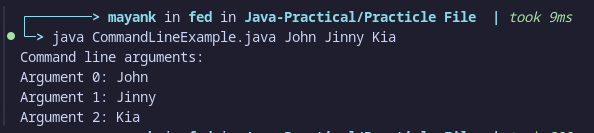
\includegraphics[width=0.9\linewidth]{images/CLA.png}
    \caption{Command Line Arguments}
    \label{fig:sample_image}
\end{figure}
\end{document}